\chapter{背景介绍}
  \section{中文拼音简介}

  目前在中国大陆,一般的学前教育或者小学教育都是选汉语拼音作为中文教育的起点。汉语拼音,或又称拼音,是一种以拉丁字母作汉字标音的方案。\supercite{wjm}汉语拼音使用拉丁字母和标注在字母之上的一些附加符号来表示汉语发音。参考现代音韵学中对汉语音节结构的划分,可以将构成汉语拼音的成分分为声母、韵母和声调三部分。现代拼音输入法主要考虑声母和韵母两部分作为检索汉字的输入。

  按照汉语拼音方案《声母表》中的规定,声母由汉语中每一个音节的起始辅音构成。在中国诸多方言中,对辅音有不同程度的混合和模糊。如西南官话中的四川方言,对卷舌音和齿龈音不加区分,部分边音与鼻音不加区分;闽南语的泉漳片方言对唇齿音和软颚音音不加区分等等。\supercite{jdp}相对的,韵母主要有汉语中没一个音节的元音构成。按照韵母结构,又可将韵母分为单韵母、复韵母和鼻韵母三类。

  在汉语拼音系统中,还有语流音变现象,包括变调、轻声、儿化、音变等等。但这些现象在现代汉语输入法中均没有得到使用,在此略过不谈。

  \section{现有输入法\label{sec:current_input}}
  现代主流的输入法种类繁多,根据,

  97\%的用户选择拼音输入法作为自己的主要输入法。\supercite{chen}

  \subsection{主流拼音输入法}

  \subsection{最新拼音输入法的新特性\label{sec:new_feature}}

  \section{现有拼音输入法的局限性\label{sec:limit}}

  \subsection{键盘布局并非最优\label{sec:layout_defect}}

  \begin{figure}[h]
  \noindent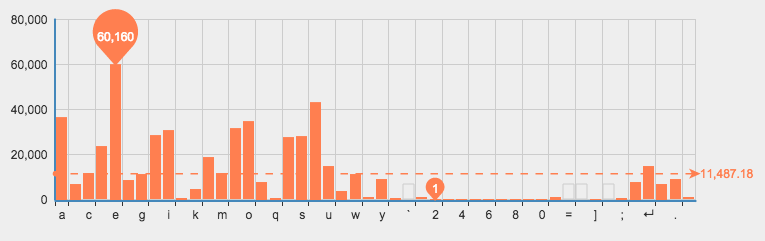
\includegraphics[width=150mm]{img/stats_en}
  \caption{英文资料键位热图}
  \label{fig:stats_en}
  \end{figure}

  \begin{figure}[h]
  \noindent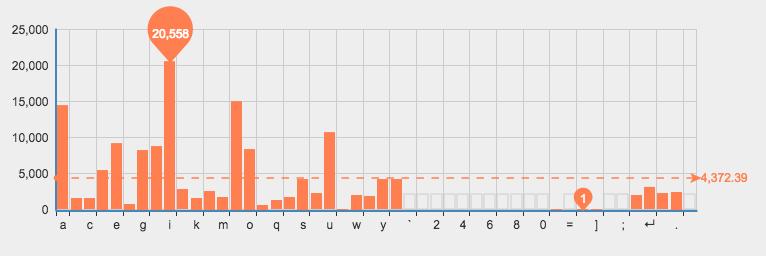
\includegraphics[width=150mm]{img/stats_cn}
  \caption{中文资料键位热图}
  \label{fig:stats_cn}
  \end{figure}
  单⼀一特征编码冗余多。键盘输⼊入法普遍采⽤用的是对汉字编码的⽅方法,即将汉字 的⾳音、形、义等特征与特定的键值相关联的编码⽅方式,但是⽬目前它们都是仅利⽤用了 汉字的⼀一⽅方⾯面特征进⾏行编码,虽然混合输⼊入法等允许⽤用户在输⼊入汉字时能够在不同 的编码⽅方式之间切换,但是某⼀一时刻仍只依据⼀一种汉字特征完成输⼊入过程,因此在 实际使⽤用中由于汉字单⼀一特征的编码存在重复编码的可能性很⼤大,所以检索到的结 果集会有较多冗余,增加了⽤用户的选择负担。对于汉语的初学者来说,通过尽可能 少的操作步骤就能将结果锁定在最⼩小的结果集中,将会促进他们的学习热情,降低 学习难度。

  回忆式操作模式门槛⾼高。键盘输⼊入法在操作上的共同特征是回忆式输⼊入⽅方式, 即⽤用户需要回忆欲输⼊入汉字的特定编码,如拼⾳音输⼊入法要求⽤用户在熟练掌握汉语拼 ⾳音的基础上记住所有汉字的拼⾳音组合,五笔输⼊入法要求⽤用户熟记键盘字母按键与特 定汉字结构的对应表等等,这⽆无疑会增加⽤用户的学习和记忆的负担,对于汉语的初 学者来说更是“望洋兴叹”。

  输⼊入错误修改繁琐。在⽇日常使⽤用中如果遇到拼写错误的情况,我们的通常⽅方法 是取消并重新输⼊入,或者使⽤用回退按键返回出错位置继续输⼊入,⽆无论哪种⽅方法都需 要进⾏行多次按键操作,影响了输⼊入的速度和连续性。

  拼⾳音声母易混淆出错概率⾼高。⽬目前所有的拼⾳音输⼊入法都是采⽤用先声母、后韵母 的⽅方式检索汉字,即要求先输⼊入声母然后输⼊入韵母的顺序,由于中国南北⽅方⾔言的差 异巨⼤大,存在相当⼀一部分⼈人⽆无法正确区分某些声母,如东北地区对zh和z、ch和c、 sh和s以及江浙地区对l和n等,并且因为包含此类声母的常⽤用汉字数量很多,这样势 必会造成⽤用户在输⼊入时频频出错,极⼤大的影响了输⼊入效率;某些⾼高级的拼⾳音输⼊入法 会在输⼊入过程中有提⽰示功能,但是由于输⼊入顺序的限制,声母⼀一旦输⼊入错误,提⽰示 的信息也不再有参考作⽤用。
